% Workflow for selecting mountain ranges comparable to the European Alps.
% Compile: pdflatex range_selection_diagram.tex
\documentclass[tikz,border=6pt]{standalone}
\usepackage[T1]{fontenc}
\usepackage{lmodern}
\usetikzlibrary{arrows.meta,positioning,calc}

\newcommand{\nohyphens}{\hyphenpenalty=10000 \exhyphenpenalty=10000 }

\begin{document}
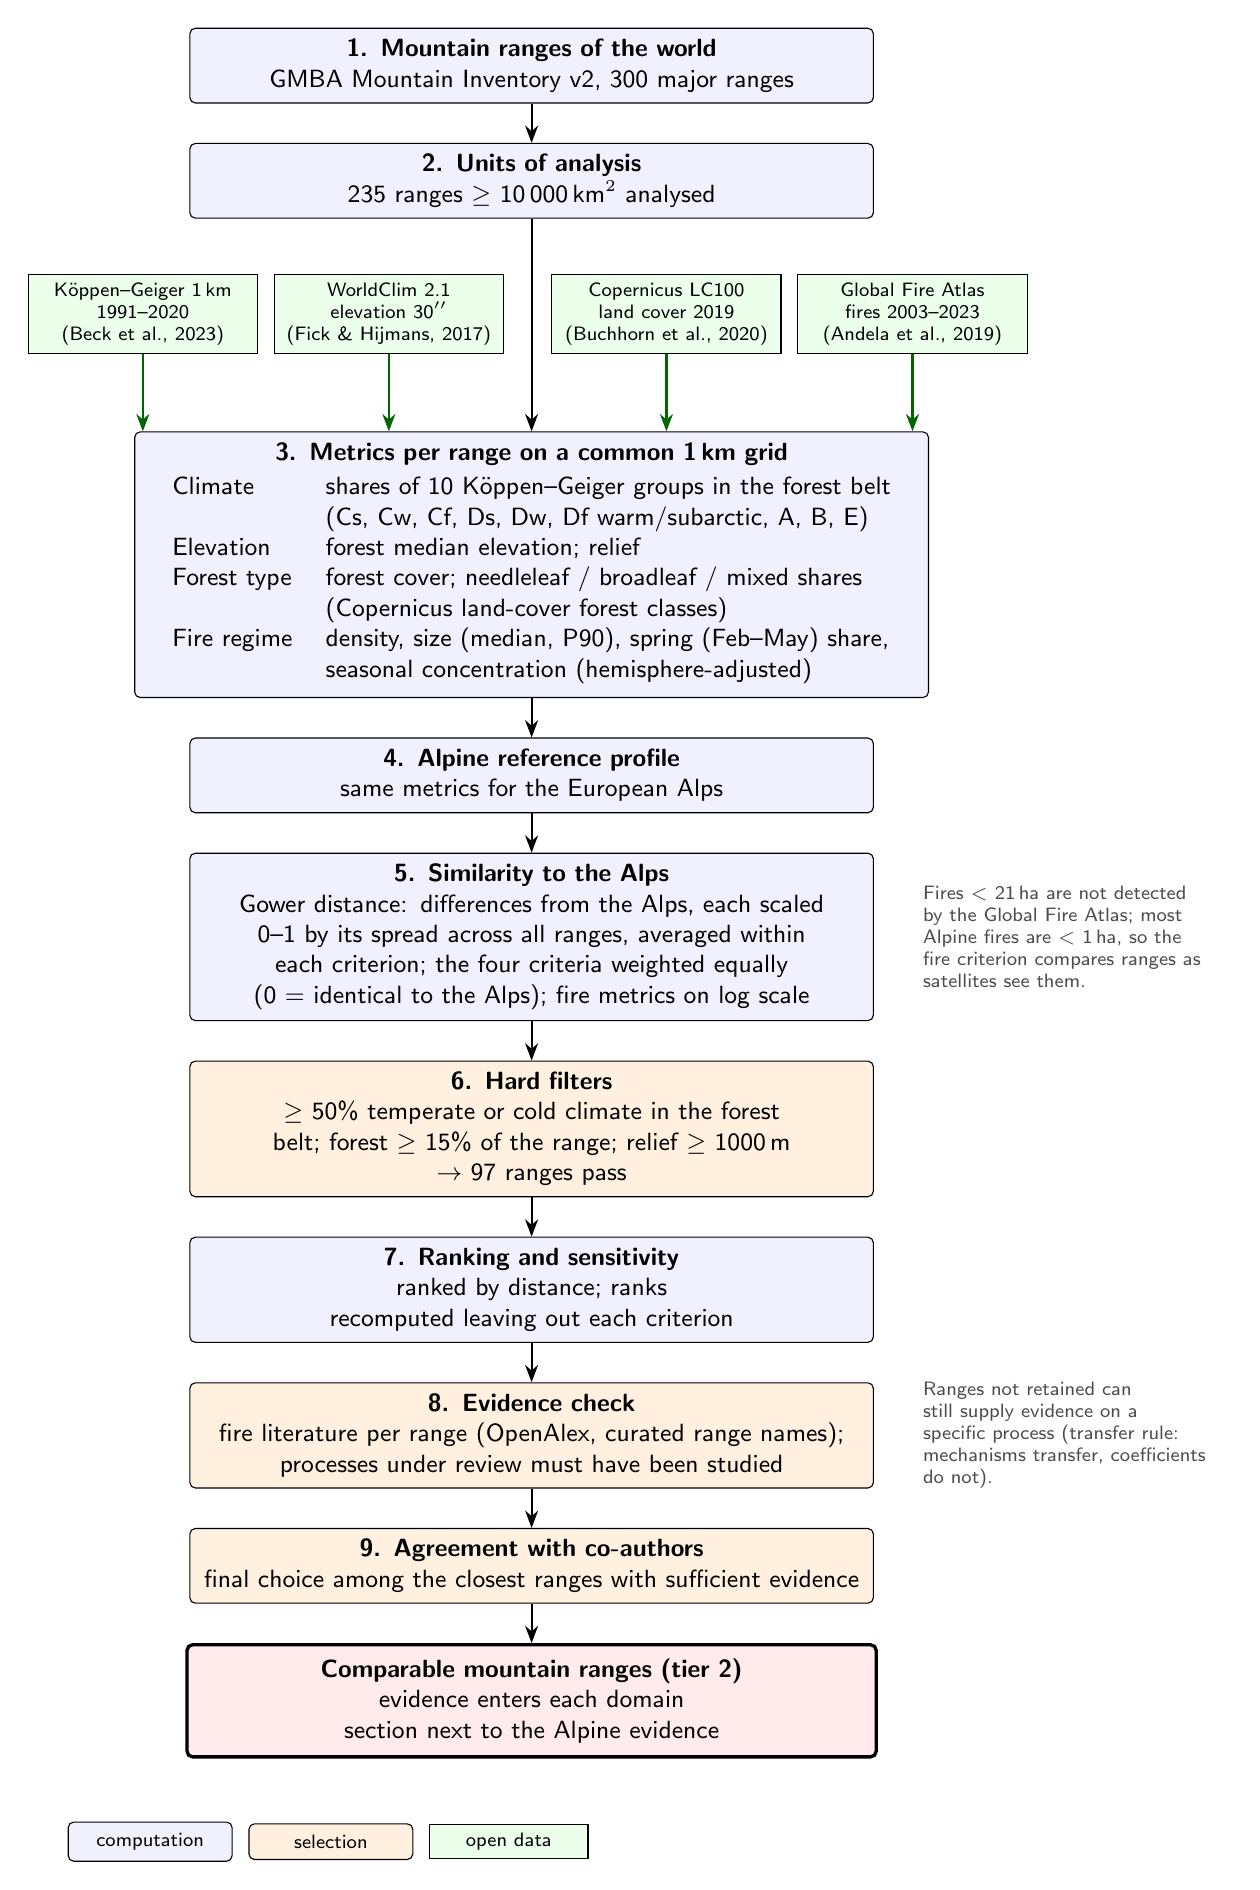
\begin{tikzpicture}[
    font=\sffamily\small,
    every node/.append style={execute at begin node=\nohyphens},
    node distance=5mm and 7mm,
    proc/.style={draw, rounded corners=2pt, fill=blue!6, align=center, text width=84mm, inner sep=4pt},
    data/.style={draw, fill=green!8, align=center, text width=27mm, inner sep=3pt, font=\sffamily\scriptsize},
    decision/.style={draw, rounded corners=2pt, fill=orange!12, align=center, text width=84mm, inner sep=4pt},
    result/.style={draw, very thick, rounded corners=2pt, fill=red!8, align=center, text width=84mm, inner sep=5pt},
    note/.style={align=left, text width=38mm, font=\sffamily\scriptsize, text=black!70},
    arrow/.style={-{Stealth[length=2.2mm]}, thick},
    ]

% Main column
\node[proc] (gmba) {\textbf{1. Mountain ranges of the world}\\
  GMBA Mountain Inventory v2, 300 major ranges};
\node[proc, below=of gmba] (size) {\textbf{2. Units of analysis}\\
  235 ranges $\geq$ 10\,000\,km$^2$ analysed};
\node[proc, text width=98mm, below=27mm of size] (metrics) {\textbf{3. Metrics per range on a common 1\,km grid}\\[2pt]
  \begin{tabular}{@{}ll@{}}
  Climate & shares of 10 Köppen--Geiger groups in the forest belt\\
          & (Cs, Cw, Cf, Ds, Dw, Df warm/subarctic, A, B, E)\\
  Elevation & forest median elevation; relief\\
  Forest type & forest cover; needleleaf / broadleaf / mixed shares\\
          & (Copernicus land-cover forest classes)\\
  Fire regime & density, size (median, P90), spring (Feb--May) share,\\
              & seasonal concentration (hemisphere-adjusted)
  \end{tabular}};
\node[proc, below=of metrics] (ref) {\textbf{4. Alpine reference profile}\\
  same metrics for the European Alps};
\node[proc, below=of ref] (gower) {\textbf{5. Similarity to the Alps}\\
  Gower distance: differences from the Alps, each scaled 0--1 by its spread across all ranges, averaged within each criterion; the four criteria weighted equally (\mbox{0 = identical} to the Alps); fire metrics on log scale};
\node[decision, below=of gower] (filter) {\textbf{6. Hard filters}\\
  $\geq$ 50\% temperate or cold climate in the forest belt;
  forest $\geq$ 15\% of the range; relief $\geq$ 1000\,m\\
  $\rightarrow$ 97 ranges pass};
\node[proc, below=of filter] (rank) {\textbf{7. Ranking and sensitivity}\\
  ranked by distance; ranks recomputed leaving out each criterion};
\node[decision, below=of rank] (lit) {\textbf{8. Evidence check}\\
  fire literature per range (OpenAlex, curated range names);\\
  processes under review must have been studied};
\node[decision, below=of lit] (agree) {\textbf{9. Agreement with co-authors}\\
  final choice among the closest ranges with sufficient evidence};
\node[result, below=of agree] (out) {\textbf{Comparable mountain ranges (tier 2)}\\
  evidence enters each domain section next to the Alpine evidence};

% Data inputs feeding step 3
\node[data, anchor=north west] (kg) at ($(size.south)+(-64mm,-7mm)$) {Köppen--Geiger 1\,km\\1991--2020\\(Beck et al., 2023)};
\node[data, right=2mm of kg] (dem) {WorldClim 2.1\\elevation 30$''$\\(Fick \& Hijmans, 2017)};
\node[data, right=6mm of dem] (lc) {Copernicus LC100\\land cover 2019\\(Buchhorn et al., 2020)};
\node[data, right=2mm of lc] (gfa) {Global Fire Atlas\\fires 2003--2023\\(Andela et al., 2019)};

% Arrows
\foreach \a/\b in {gmba/size, size/metrics, metrics/ref, ref/gower, gower/filter, filter/rank, rank/lit, lit/agree, agree/out}
  \draw[arrow] (\a) -- (\b);
\foreach \d in {kg, dem, lc, gfa}
  \draw[arrow, green!40!black] (\d.south) -- (\d.south |- metrics.north);

% Side notes
\node[note, right=5mm of gower] {Fires $<$ 21\,ha are not detected by the Global Fire Atlas;
  most Alpine fires are $<$ 1\,ha, so the fire criterion compares ranges as satellites see them.};
\node[note, right=5mm of lit] {Ranges not retained can still supply evidence on a specific process
  (transfer rule: mechanisms transfer, coefficients do not).};

% Legend
\node[proc, text width=18mm, font=\sffamily\scriptsize, below left=8mm and -6mm of out] (lg1) {computation};
\node[decision, text width=18mm, font=\sffamily\scriptsize, right=2mm of lg1] (lg2) {selection};
\node[data, text width=18mm, right=2mm of lg2] (lg3) {open data};
\end{tikzpicture}
\end{document}
